\chapter{Diseño}
En esta sección se describirá el diseño de la plataforma \textbf{GAC} (Gestor Académico de Calendarios). Se detallarán los aspectos más relevantes de la arquitectura, la interfaz de usuario y la base de datos.



\section{Arquitectura software}
La arquitectura software se refiere a la vista del sistema que incluye los componentes principales del mismo, la conducta de dichos componentes según se la percibe desde el resto del sistema y las formas en las que interactúan y se coordinan entre sí para lograr los objetivos del sistema. Sus dos principales aspectos son, que provee de un plan de diseño, un ``blueprint'' del sistema a la vez que hace de abstracción del mismo para ayudar a manejar la complejidad del mismo. Una buena arquitectura software es el garante de un sistema que cumple con los requisitos de calidad, como la eficiencia, la fiabilidad, la seguridad, la mantenibilidad, la escalabilidad, la portabilidad, la usabilidad, la interoperabilidad, la disponibilidad y la capacidad de evolución \cite{hofmeister2000applied, reynoso2004introduccion, garlan2008software}.\newline

Para el desarrollo de la plataforma se ha optado por una arquitectura cliente-servidor basada en una Arquitectura Orientada a Servicios (SOA). La API\footnote{\url{https://aws.amazon.com/es/what-is/api/}} ha sido desarrollada en Python y Flask y se encarga de manejar las solicitudes del cliente. Todo lo mencionado puede verse en la Figura \ref{fig:soa}.\newline

\newpage

Adicionalmente, se ha desarrollado un web scraper\footnote{\url{https://kinsta.com/es/base-de-conocimiento/que-es-web-scraping/}} que se encarga de obtener toda la programación docente de la oficina virtual de la Universidad de Granada\footnote{\url{https://oficinavirtual.ugr.es}}. Los usuarios realizan peticiones desde la plataforma web al servidor, el cual se encarga de procesarlas y devolver una respuesta.\newline


\subsection{Arquitectura cliente-servidor}

La arquitectura cliente-servidor (Figura \ref{fig:cliente_servidor}) es un modelo de diseño de software en el que las tareas se reparten entre los proveedores de recursos o servicios, llamados \textbf{servidores}, y los demandantes, llamados \textbf{clientes}. Un cliente realiza una petición a un servidor, el cual procesa la solicitud y devuelve una respuesta. La comunicación entre ambos se realiza a través de una red, generalmente utilizando el protocolo TCP/IP. Actualmente, se emplea el término backend para referirse a los servidores y frontend para los clientes.\newline

\begin{figure}[H]
    \centering
    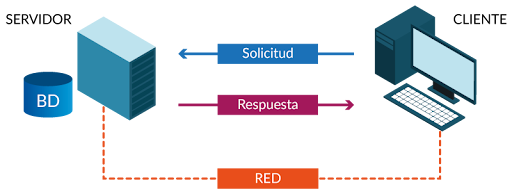
\includegraphics[width=0.7\textwidth]{./imagenes/cliente_servidor.png}
    \caption{Arquitectura Cliente-Servidor \cite{sucerman2023}.}
    \label{fig:cliente_servidor}
\end{figure}

\subsubsection*{Cliente}

El cliente es la parte del sistema que interactúa con el usuario final. Se encarga de enviar solicitudes al servidor y de procesar la respuesta para mostrarla al usuario. Puede ser una aplicación de escritorio, una aplicación web o una aplicación móvil. En el caso de la plataforma \textbf{GAC}, el cliente es una aplicación web que se ejecuta en un navegador.\newline

\subsubsection*{Servidor}

El servidor es la parte del sistema que recibe las solicitudes del cliente, las procesa y devuelve una respuesta. Puede ser un servidor web, un servidor de bases de datos o un servidor de aplicaciones. En el caso de la plataforma \textbf{GAC}, el servidor es un contenedor de Docker que se encarga de gestionar las solicitudes de los clientes y de comunicarse con la base de datos.

\subsubsection*{Ventajas e inconvenientes}

Las ventajas de la arquitectura cliente-servidor son varias, garante de ello es su amplia adopción en la industria del software. Entre las más destacadas se encuentran:

\begin{itemize}
    \item [$\circ$] Facilidad en la administración y control de los datos al encontrarse los recursos en entornos de servidor controlados
    \item [$\circ$] Escalabilidad, ya que se pueden ampliar ambos entornos, centrando las necesidades de escalabilidad en el servidor.
    \item [$\circ$] Permite el mantenimiento individual de las capas software, lo que permite aislar problemas y facilitar la corrección de errores.
    \item [$\circ$] Desarrollo menos dependiente, ya que se pueden desarrollar las capas de forma separada.
\end{itemize}

Sin embargo, también presenta inconvenientes, como la necesidad de una infraestructura de red para la comunicación entre cliente y servidor, la dependencia de la disponibilidad del servidor y la necesidad de una mayor seguridad en la comunicación entre ambos.\newline


\subsection{Arquitectura Orientada a Servicios (SOA)}

La Arquitectura Orientada a Servicios\footnote{\url{https://www.redhat.com/es/topics/cloud-native-apps/what-is-service-oriented-architecture}} es un tipo de diseño de software que permite reutilizar sus elementos gracias a las interfaces de servicios que se comunican a través de una red con un lenguaje común (Figura \ref{fig:soa_stack}). Un servicio es una unidad autónoma de una o más funciones software, diseñada para realizar una tarea específica, como recuperar cierta información o ejecutar una operación.\newline

\begin{figure}[H]
    \centering
    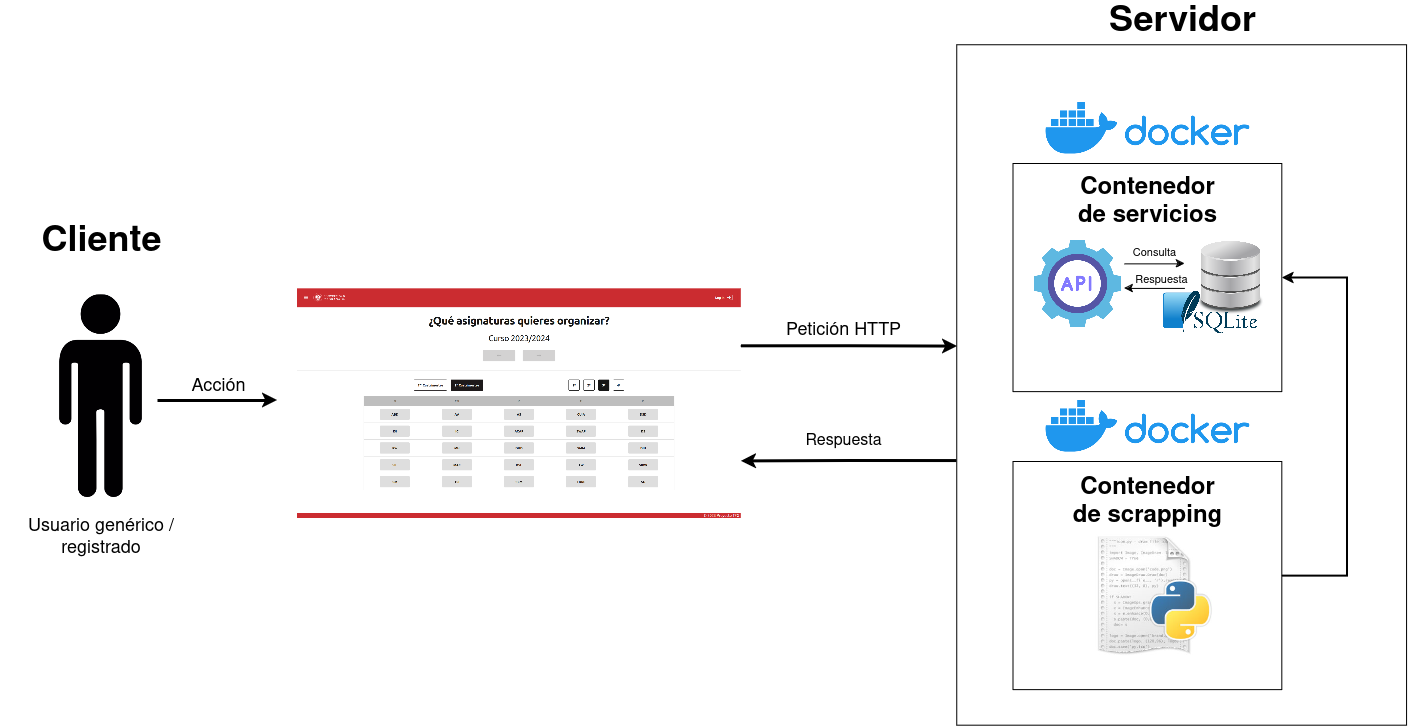
\includegraphics[width=1\textwidth]{./imagenes/Arq_Soft_informal.png}
    \caption{Arquietctura Orientada a Servicios basada en Cliente-Servidor.}
    \label{fig:soa}
\end{figure}

Desde la perspectiva de quien lo invoca, es vista como una funcionalidad autocontenida que encapsula su implementación, por tanto, \textbf{no es necesario saber como está implementado} o como funciona internamente, \textbf{solo es fundamental saber cómo se usa} y qué se espera de él. En resumen, un servicio es una interfaz que se expone a través de una red y que se puede invocar para realizar una tarea específica, como puede verse en la Figura \ref{fig:soa_interface}.\newline

\begin{figure}[H]
    \centering
    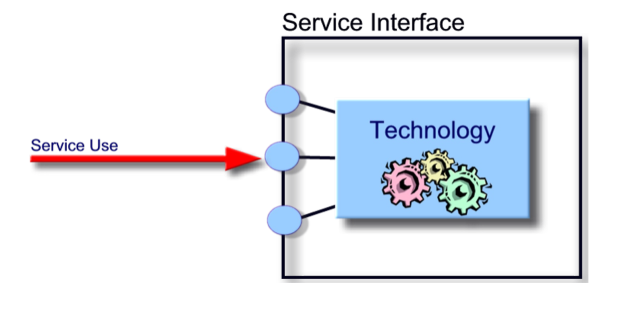
\includegraphics[width=0.7\textwidth]{./imagenes/Interfaz_SOA.png}
    \caption{Servicio como interfaz.}
    \label{fig:soa_interface}
\end{figure}

Dado que SOA expone los servicios utilizando protocolos estándar de red para enviar solicitudes o acceder a los datos, se facilita la interoperabilidad entre diferentes sistemas y la atomicidad desde la perspectiva del usuario \cite{laskey2009service, 1210138}. Los servicios pueden componerse, constituyendo lo que se conoce como ``building blocks'' y facilitando su reutilización para desarrollar otras aplicaciones. El enfoque está en sus interfaces, no en su implementación, lo que permite a los servicios ser utilizados de forma agnóstica a su ubicación y tecnología.\newline

Hay dos formas de componer servicios en SOA (Figura \ref{fig:soa_composition}):

\begin{itemize}
    \item \textbf{Orquestación:} Se construyen funcionalidades más complejas a partir de servicios más simples, mientras que el flujo de control es manejado por un motor de orquestación.
    \item \textbf{Coreografía:} Los servicios complejos compuestos por servicios simples colaboran entre sí para lograr un objetivo común, sin un motor de orquestación central.
\end{itemize}

\begin{figure}[H]
    \centering
    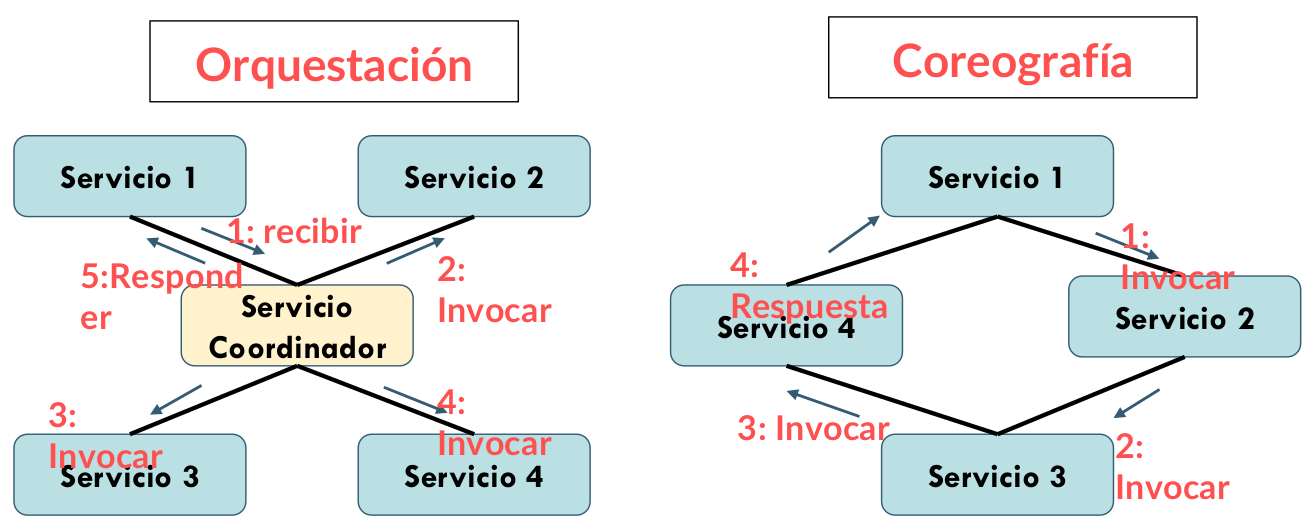
\includegraphics[width=1\textwidth]{./imagenes/Orquestacion_y_coreografia.png}
    \caption{Composición de servicios en SOA.}
    \label{fig:soa_composition}
\end{figure}

Bajo el marco de una arquitectura cliente-servidor, las llamadas a los servicios se realizan mediante el protocolo HTTP y la información de respuesta se devuelve en formato JSON, estándar en la intercomunicación de esta arquitectura.\newline

\begin{figure}
    \centering
    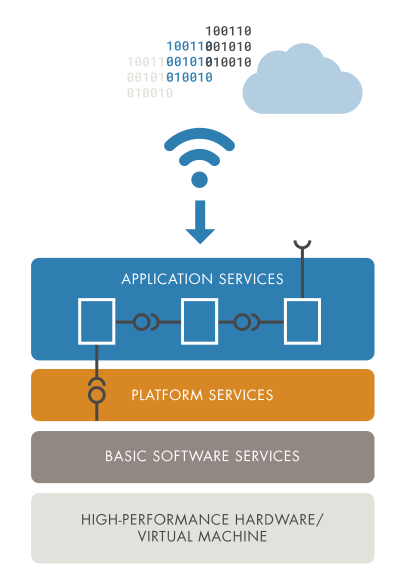
\includegraphics[width=0.5\textwidth]{./imagenes/SOA.png}
    \caption{Pila de software SOA generalizada \cite{soa}.}
    \label{fig:soa_stack}
\end{figure}

\subsubsection{Principios de SOA}

\begin{itemize}
    \item \textbf{Contratos de servicio estandarizados:}
    \begin{itemize}
        \item[$\circ$] Para que se considere un servicio, su contrato con el cliente, es decir, la interfaz que expone, debe estar explícitamente declarada.
        \item[$\circ$] Los campos que forman la interfaz deben ser tipados y conocidos.
        \item[$\circ$] Todos usan el servicio de la misma manera.  
    \end{itemize}
    \item \textbf{Servicios con bajo acoplamiento:}
    \begin{itemize}
        \item[$\circ$] Debe haber baja dependencia entre los servicios.
        \item[$\circ$] A menor acoplamiento, mayor independencia.
        \item[$\circ$] Mejor diseño del servicio. 
    \end{itemize}
    \item \textbf{Abstracción:}
    \begin{itemize}
        \item[$\circ$] Los detalles internos del servicio deben estar ocultos.
        \item[$\circ$] El servicio debe ser visto como una caja negra, solo se conoce su interfaz.
        \item[$\circ$] La interfaz es el mínimo acoplamiento posible con el consumidor.
    \end{itemize}
    \item \textbf{Reusabilidad:}
    \begin{itemize}
        \item [$\circ$] No busca la sustitución de las lógicas de negocio actuales, sino que busca proporcionar una forma de aprovechar estos activos, encapsulándolos en servicios para que estos a su vez puedan ser reutilizados por otros servicios.
    \end{itemize}
    \item \textbf{Autonomía:}
    \begin{itemize}
        \item [$\circ$] El servicio debe tener un alto grado de control sobre su propio entorno de ejecución y la lógica que encapsula.
    \end{itemize}
    \item \textbf{Sin estado:}
    \begin{itemize}
        \item [$\circ$] Idealmente, todos los datos que necesita el servicio provienen sus parámetros de entrada.
        \item [$\circ$] El tratamiento de una gran información de estado repercutiría en la escalabilidad del servicio.
    \end{itemize}
    \item \textbf{Descubrimiento:}
    \begin{itemize}
        \item [$\circ$] Al servicio se le dotarán de metadatos que permitan su descubrimiento de manera efectiva.
        \item Estos metadatos pueden ser interpretados y reutilizados de manera automática.
        \item Para ello, se requiere disponer de un mecanismo de descubrimiento como el \textbf{UDDI} (Universal Description, Discovery and Integration) \footnote{\url{https://www.ibm.com/docs/es/rsm/7.5.0?topic=standards-universal-description-discovery-integration-uddi}}.
    \end{itemize}
    \item \textbf{Composición:}
    \begin{itemize}
        \item [$\circ$] Los servicios pueden ser compuestos para formar servicios más complejos.
        \item [$\circ$] A medida que la arquitectura SOA se consolide, los servicios son elegibles de componerse en nuevos servicios más complejos (de alto nivel).
        \item [$\circ$]La implementación de nuevos servicios se reducirá al mínimo y los nuevos servicios se compondrán de servicios ya existentes.
    \end{itemize}
\end{itemize}

\section{Diseño Lógico}

Los diagramas de clase UML (Unified Modeling Language) son el núcleo del diseño y análisis orientado a objetos y son una forma de modelar la estructura estática de un sistema, por medio de clases, atributos, métodos y relaciones entre ellas \cite{herchi2012user}. Todas las clases del diagrama que se muestra en la Figura \ref{fig:class_diagram}, se traducirán a tablas donde sus campos serán los atributos que se detallan en la figura. A continuación se muestra el diagrama de clases y secuencia de la plataforma.\newline

Adicionalmente, se ha desarrollado un diagrama de secuencia que muestra la interacción entre los diferentes componentes de la plataforma. En este diagrama se puede observar cómo se realiza la comunicación entre los diferentes elementos de la plataforma como puede verse en la Figura \ref{fig:sequence_diagram}.\newline

\newpage

\begin{landscape}
    \begin{figure}[H]
        \centering
        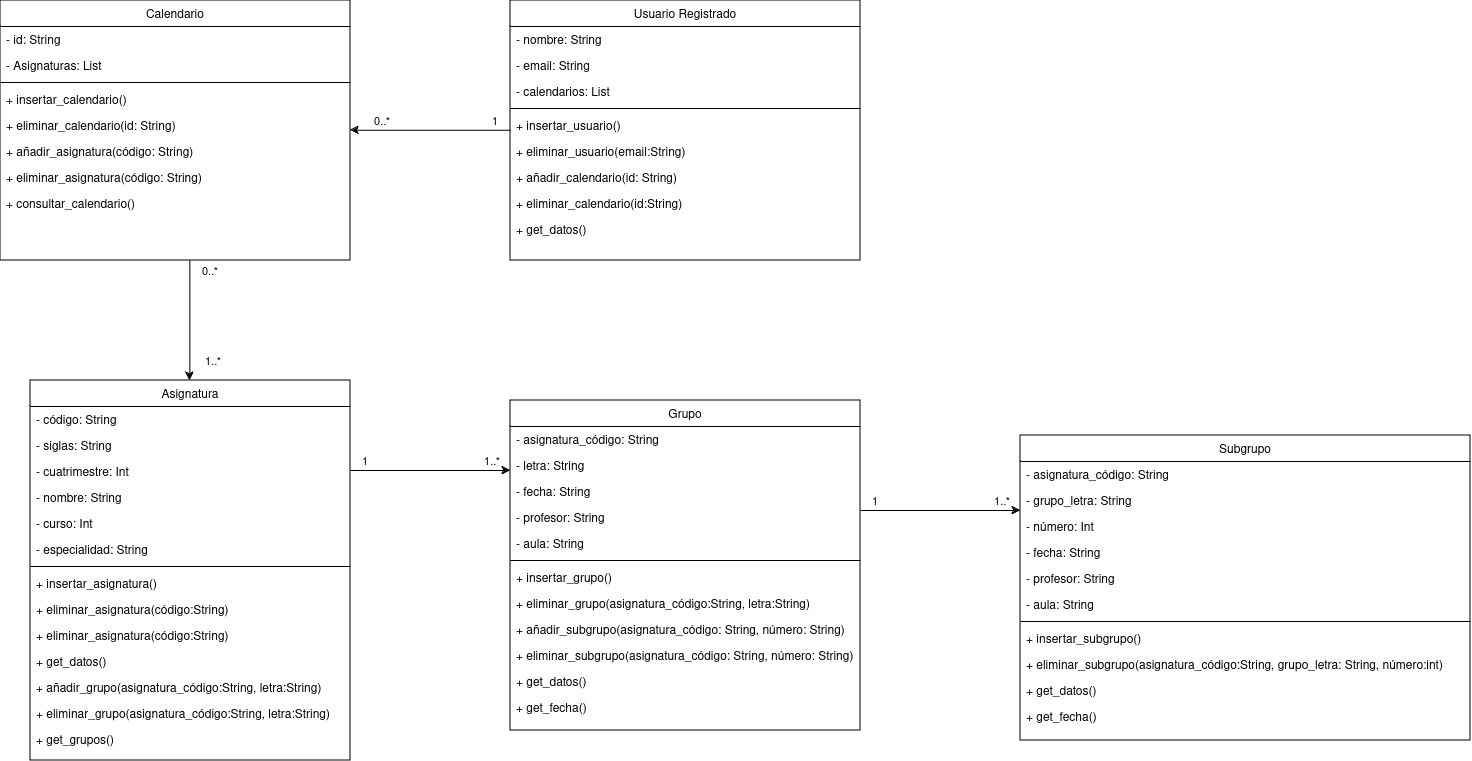
\includegraphics[width=1.6\textwidth]{./imagenes/Class_Diagram.png}
        \caption{Diagrama de clases de la plataforma.}
        \label{fig:class_diagram}
    \end{figure}  
\end{landscape}

\begin{landscape}
    \begin{figure}[H]
        \centering
        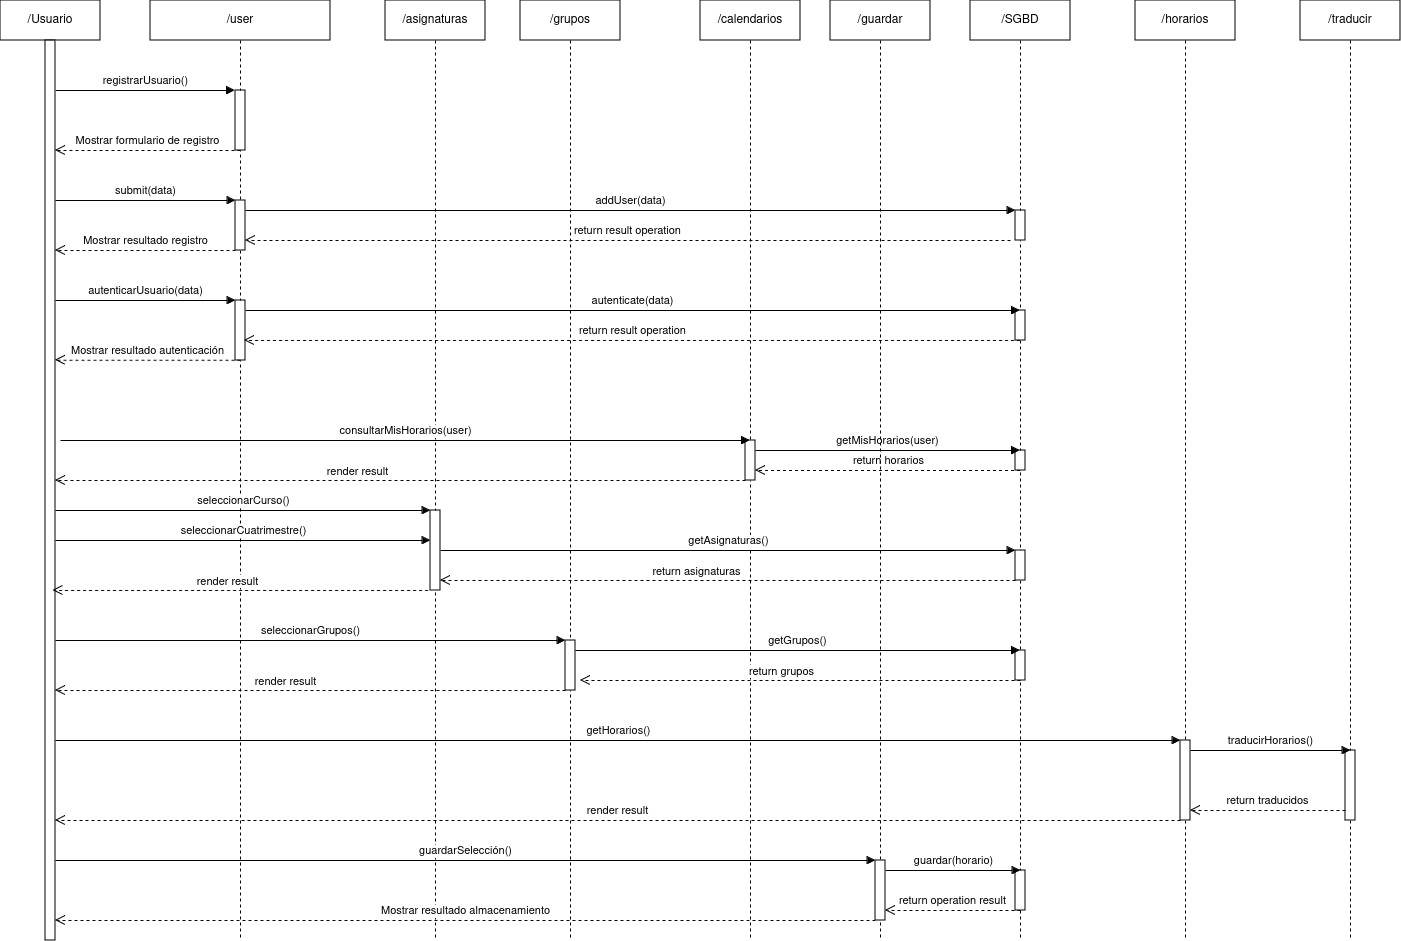
\includegraphics[width=1.35\textwidth]{./imagenes/Secuencia_Diagrama.png}
        \caption{Diagrama de secuencia de la plataforma.}
        \label{fig:sequence_diagram}
    \end{figure}    
\end{landscape}

\section{Diseño de Wireframes para Frontend}

Un wireframe\footnote{\url{https://miro.com/es/wireframe/que-es-wireframe/}} es un diagrama visual que esboza el esqueleto de un proyecto o pieza tecnológica. Los diseñadores de UX (User Experience) suelen utilizarlo para trazar el diseño y la composición de su trabajo si entrar en detalles de paletas de color, etc. Es la etapa previa a los mockups y prototipos y se caracterizan por la ausencia de colores y elementos de diseño estético.\newline

Los wireframes que se muestra en las Figuras \ref{fig:wireframe_a} y \ref{fig:wireframe_b}, pertenecen a los primeros bocetos de la interfaz de usuario de la plataforma \textbf{GAC}, realizados con la plataforma Moqups \footnote{\url{https://moqups.com/es/}}. En las primeras etapas del diseño se consideró el uso de modelos de IA generativa para el desarrollo de los calendarios. Además, se pretendía que la plataforma fuese una especie de organizador personal tipo Google Calendar. Pueden consultarse el resto de diseños en el Anexo I.\newline


\begin{figure}[H]
    \centering
    \begin{subfigure}[b]{0.51\textwidth}
        \centering
        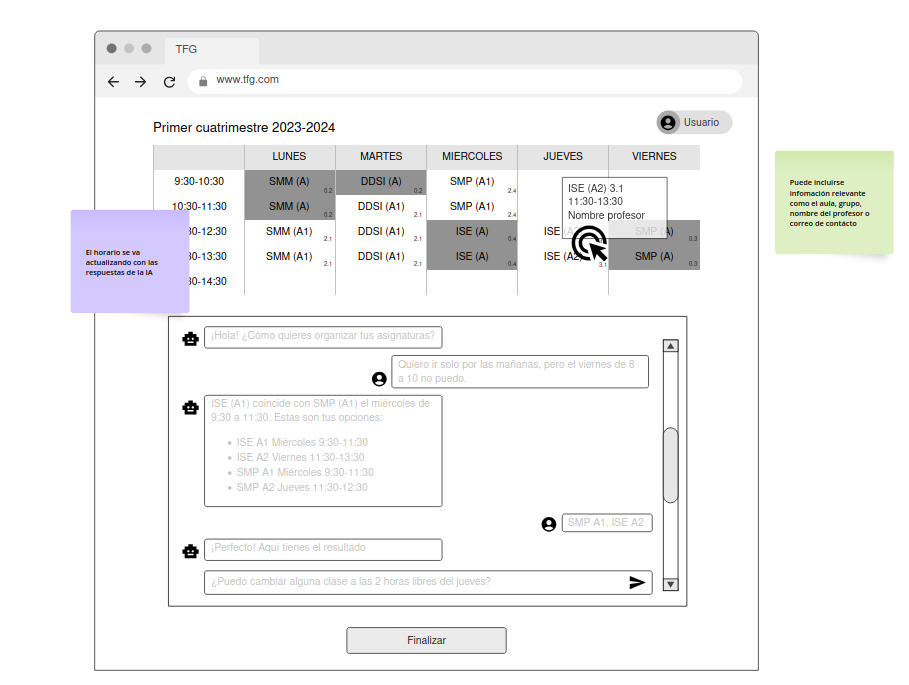
\includegraphics[width=\textwidth]{./imagenes/Mockup_calendario.png}
        \caption{Calendario académico con chat de asistente.}
        \label{fig:wireframe_a}
    \end{subfigure}
    \hfill
    \begin{subfigure}[b]{0.48\textwidth}
        \centering
        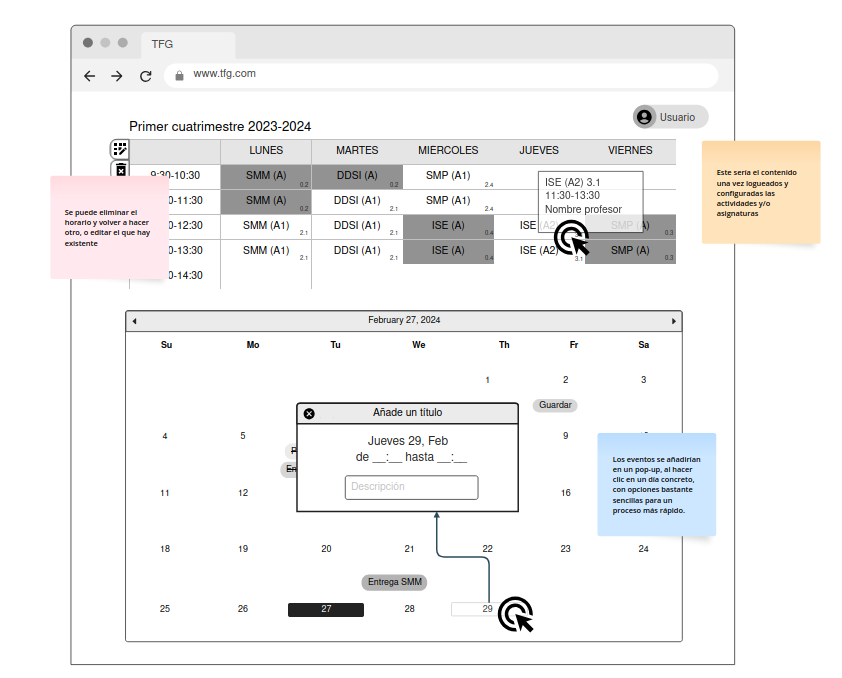
\includegraphics[width=\textwidth]{./imagenes/Mockup_organizador.png}
        \caption{Calendario académico y mensual de actividades.}
        \label{fig:wireframe_b}
    \end{subfigure}
    \caption{Wireframes de la interfaz de usuario.}
\end{figure}



